\documentclass[a4paper]{article}
\usepackage[a4paper,top=2cm,bottom=2cm,left=1cm,right=1cm,marginparwidth=1.75cm]{geometry}
% \usepackage[spanish]{babel}
% \selectlanguage{spanish}
% \usepackage[utf8]{inputenc}
% \usepackage[T1]{fontenc}
% \usepackage[spanish]{babel}

% \usepackage[T1]{fontenc}
\usepackage{graphicx} %Paquete para usar imagenes
\usepackage{listings}
\usepackage{xcolor}
\usepackage{tcolorbox}\usepackage{hyperref}

\definecolor{background}{HTML}{E7EBF4}
\definecolor{bg}{HTML}{1a1b26}
\definecolor{fg}{HTML}{a9b1d6}
\definecolor{comment}{HTML}{848cb5}
\definecolor{cyan}{HTML}{82aaff}
\definecolor{orange}{HTML}{ff9e64}
\definecolor{yellow}{HTML}{e9d78e}
\definecolor{purple}{HTML}{c792ea}
\definecolor{green}{HTML}{7fdbca}
\definecolor{numbers}{HTML}{9854f1}
\definecolor{keyword}{HTML}{9854f1}

\lstset{
    showspaces=false, % Evita mostrar espacios en blanco como ␣
    showstringspaces=false,
    inputencoding=utf8,
    extendedchars=true,
    literate=%
    {á}{{\'a}}1
    {é}{{\'e}}1
    {í}{{\'i}}1
    {ó}{{\'o}}1
    {ú}{{\'u}}1
    {ñ}{{\~n}}1
}
\lstdefinestyle{mystyle}{
    language=sql,
    basicstyle=\ttfamily,
    keywordstyle=\color{keyword},
    commentstyle=\color{comment},
    numbers=none,
    numberstyle=\tiny\color{numbers},
    frame=none,
    breaklines=true,
    % showstringspaces=false
    xleftmargin=0mm,
    xrightmargin=0mm,
}

\lstset{style=mystyle}

\newtcolorbox{mycodebox}[1][]{
    arc=17pt,  % Radio de las esquinas redondeadas
    colback=background,  % Color de fondo del cuadro
    boxrule=0.5pt,  % Grosor de la línea del cuadro
    colframe=background,
    width=0.8\textwidth,   % Anchura del cuadro
    % height=5cm,            % Altura del cuadro
    % breakable,
    #1  % Otras opciones personalizadas que puedas necesitar
}


\newtcolorbox{mycodeboxl}[1][]{
    arc=7pt,  % Radio de las esquinas redondeadas
    colback=background,  % Color de fondo del cuadro
    boxrule=0.5pt,  % Grosor de la línea del cuadro
    colframe=background,
    width=0.94\textwidth,   % Anchura del cuadro
    % height=5cm,            % Altura del cuadro
    % breakable,
    #1  % Otras opciones personalizadas que puedas necesitar
}

% Documento
\begin{document}
\newgeometry{left=3cm,right=3cm,top=2cm,bottom=2cm}
\begin{titlepage}

%--------------- Nuevo comendo de linea ----------------->
\newcommand{\linea}{\rule{\linewidth}{0.7mm}} 
\center
%--------------- Universidad, facultad y carrera ----------------->
\textbf{\Large UNIVERSIDAD NACIONAL DE SAN ANTONIO ABAD DEL CUSCO}\\[0.2cm]
\textbf{\Large FACULTAD DE INGENIERÍA ELÉCTRICA, ELECTRÓNICA,INFORMÁTICA Y MECÁNICA}\\[0.2cm]
\textbf{\Large INGENIERÍA INFORMÁTICA Y DE SISTEMAS\\[0.6cm]}

%--------------- Escudos png ----------------->

\includegraphics[width=8cm]{src/escudo-unsaac.png}
\vfill

%--------------- Tema ----------------->
\linea
\\[0.3cm]
% \vfill
\textbf{\LARGE Guía de Laboratorio 6 - Uso de Cursores}\\[0.2cm]
\linea \\
\vfill

%--------------- Integrantes ----------------->
\textit{\Large Alumno:}\\
%Integrantes del grupo
    \textbf{\large Ian Logan Will Quispe Ventura}\\
    \textit{211359}\\
    % \vfill

%--------------- Profesor y curso ----------------->
\vspace{0.3cm}
    \textit{\Large Docente:}\\
    \textbf{\large Karelia Medina Miranda}\\
\vspace{0.5cm}
    \textit{\Large Curso:}\\
    \textbf{\large Fundamentos y Diseño de Base de Datos}\\
    \vfill

\vspace{0.4cm}
    \textbf{\Large Cusco - Perú }\\
    \textbf{\large 2023 - II }\\
    \newpage
    \end{titlepage}

\restoregeometry
\newpage
% •·•·•·•·•·•••·•·•·•·•·•·•·•·•·•·•·•·•·•·•·•·•·•·•·•·•.,..,
% \section{Funcionamiento del algoritmo DDA}

\Large{\textbf{Ejercicio Número 2}}\\
Determinar la relación de los tres prestatarios rurales más representativos de cada comunidad. Los más representativos son los que tienen mayor número de préstamos.
\begin{center}
\begin{mycodeboxl}
\begin{lstlisting}
begin
declare @CodComunidad varchar(12);
declare @CodPrestatario varchar(12);
declare @NombrePrestatario varchar(40);
declare @NumPrestamos int;

-- Crear una tabla temporal para almacenar los resultados
create table #Resultados (
    CodComunidad varchar(12),
    CodPrestatario varchar(12),
    NombrePrestatario varchar(40),
    NumPrestamos int);

-- Declarar cursor para comunidades
declare cursor_Comunidad cursor
for
select CodComunidad from Comunidad;
open cursor_Comunidad;

-- Recorrer comunidades
fetch next from cursor_Comunidad into @CodComunidad;
while @@FETCH_STATUS = 0
begin
    -- Cursor que contará los préstamos de cada prestatario en cada comunidad
    declare cursor_Prestatario cursor
    for
    select P.CodPrestatario, Pr.Nombres, count(*) as NumPrestamos
    from Prestamo P
    join Prestatario Pr on P.CodPrestatario = Pr.CodPrestatario
    where Pr.CodComunidad = @CodComunidad
    group by P.CodPrestatario, Pr.Nombres;
\end{lstlisting}
\end{mycodeboxl}
\end{center}
% -------------------------------------------------------------------
\newpage
\begin{center}
\begin{mycodeboxl}
\begin{lstlisting}
    open cursor_Prestatario;
    -- Recorremos cada uno de los prestatarios para seleccionar los tres con mayor número de préstamos
    declare @Counter int = 0;
    fetch next from cursor_Prestatario into @CodPrestatario, @NombrePrestatario, @NumPrestamos;
    while @@FETCH_STATUS = 0 and @Counter < 3
    begin
        -- Guardamos los resultados obtenidos en la tabla temporal
        insert into #Resultados (CodComunidad, CodPrestatario, NombrePrestatario, NumPrestamos)
        values (@CodComunidad, @CodPrestatario, @NombrePrestatario, @NumPrestamos);

        set @Counter = @Counter + 1;
        -- Siguiente prestatario
        fetch next from cursor_Prestatario into @CodPrestatario, @NombrePrestatario, @NumPrestamos;
    end;
    close cursor_Prestatario;
    deallocate cursor_Prestatario;
    -- Siguiente comunidad
    fetch next from cursor_Comunidad into @CodComunidad;
end;

close cursor_Comunidad;
deallocate cursor_Comunidad;
select * from #Resultados;
-- Eliminar la tabla temporal
drop table #Resultados;
end;

\end{lstlisting}
\end{mycodeboxl}
\end{center}
\newpage
Resultados 
\begin{center}
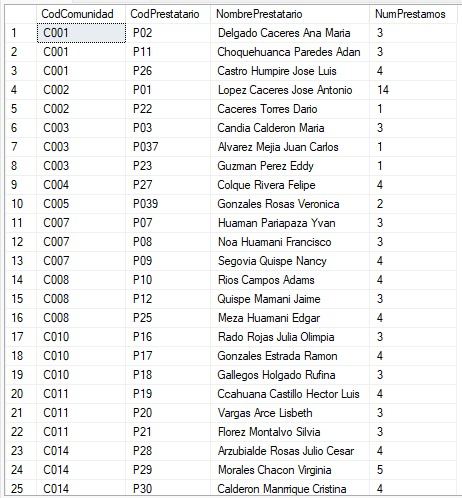
\includegraphics[width=16cm]{./src/1.jpeg}
\end{center}
% -------------------------------------------------------------------
\newpage
\Large{\textbf{Problema Número 3}}\\
Determinar los movimientos de un prestatario. Debe mostrar cada préstamo con sus respectivas cancelaciones. Los importes del préstamo van en la columna del Debe y los importes de las cancelaciones van al haber. Considerar que un prestatario puede tener varios préstamos.
\begin{center}
\begin{mycodeboxl}
\begin{lstlisting}
begin
declare @CodPrestatario TCodPrestatario;
set @CodPrestatario = 'P01';

-- Crear tabla para almacenar los movimientos de los prestatarios
create table #Movimientos (
    DocMovimiento varchar(12),
    FechaMovimiento datetime,
    Debe numeric(15,2),
    Haber numeric(15,2),
    SaldoPrestado numeric(15,2),
    SaldoTotal numeric(15,2)
);

-- Declarar variables
declare @SaldoPrestado numeric(15,2) = 0;
declare @SaldoTotal numeric(15,2) = 0;

-- Obtener préstamos y cancelaciones del prestatario
insert into #Movimientos
select P.DocPrestamo as DocMovimiento,
       P.FechaPrestamo as FechaMovimiento,
       P.Importe as Debe, 0 as Haber,
       P.Importe as SaldoPrestado,
       @SaldoTotal + P.Importe as SaldoTotal

from Prestamo P
where P.CodPrestatario = @CodPrestatario
order by P.FechaPrestamo;
\end{lstlisting}
\end{mycodeboxl}
\end{center}
% -------------------------------------------------------------------
\newpage
\begin{center}
\begin{mycodeboxl}
\begin{lstlisting}
insert into #Movimientos
select A.DocCancelacion as DocMovimiento,
       A.FechaCancelacion as FechaMovimiento,
       0 as Debe, A.Importe as Haber,
       -A.Importe as SaldoPrestado,
       @SaldoTotal - A.Importe as SaldoTotal

from Amortizacion A
where A.DocPrestamo in (select P.DocPrestamo
    from Prestamo P where P.CodPrestatario = @CodPrestatario)
order by A.FechaCancelacion;

select * from #Movimientos;
drop table #Movimientos;
end;
\end{lstlisting}
\end{mycodeboxl}
\end{center}
\newpage
Resultados 
\begin{center}
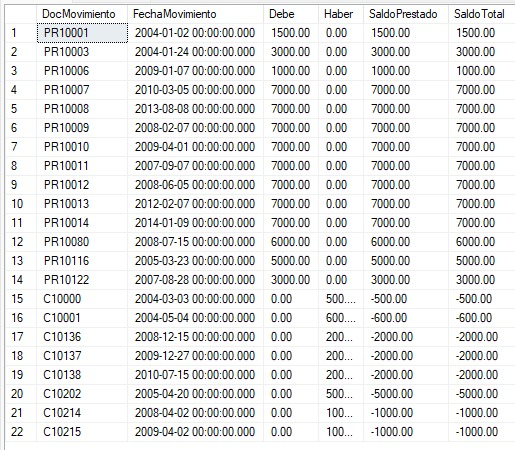
\includegraphics[width=16cm]{./src/2.jpeg}
\end{center}
\newpage
% -------------------------------------------------------------------
\end{document}
